% 第3章 関連研究
\newpage
%自分の研究との比較が可能なものだけ関連研究に載せる
\renewcommand{\baselinestretch}{1.5}
\section{関連研究}
\renewcommand{\baselinestretch}{1}
\par 近年画像解析技術の進歩により風景などの自然画像の顕著性マップ生成モデルに関する研究は多くされているが、ウェブページに特化した顕著性マップ生成モデルに関する研究はほとんど存在しない。

\subsection{自然画像の顕著性マップ生成モデル}\label{subsec:related-01}
\par 自然画像の顕著性を計算するモデルは昔から研究されて様々なモデルが存在する。中でも基本的な顕著性マップ生成モデルとしてItti-Kochらの顕著性モデル\cite{itti1998model}は広く知られている。このモデルでは、人間の目の視覚認識と同様に色・輝度・方向のそれぞれの視覚特徴を抽出した後に重み付けして足し合わせることにより顕著性マップを生成するモデルである。図\ref{fig_itti-kochi}に計算モデルの構造を示す。このモデルは視覚的顕著性に関連性のある数多くの研究で利用されている。

\begin{figure}[H]
    \centering
    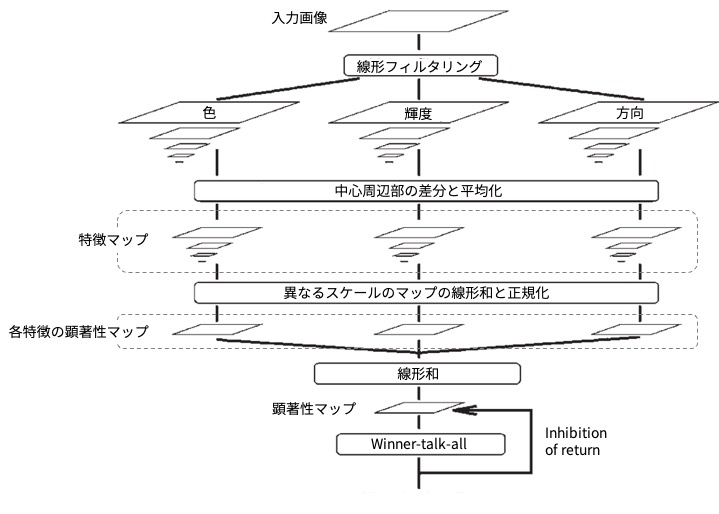
\includegraphics[width=8.5cm]{figures/itti-kochi-model.jpg}
    \caption{Itti-Kochらによる顕著性計算モデルの構造\cite{itti1998model}\label{subsec:related-01}}
    \label{fig_itti-kochi}
\end{figure}

\par 近年の技術の進歩により大規模なデータセットからトレーニングされたディープラーニング手法を活用したモデルが多く研究されている。PanらによるSalNet\cite{pan2016shallow}では顕著度を最初から予測するために独自の畳み込みニューラルネットワーク(CNN)を学習して構築された。また、学習済みの畳み込みニューラルネットワークを使用する事でJiangらによるSALICON\cite{jiang2015salicon}やCorniaらによるML-NET\cite{Cornia_2018}やKummererらによるDeep Gaze 2\cite{kummerer2016deepgaze}などの自然画像向けの顕著性マップ生成モデルを構築されている。KummererらはMITの顕著性マップのベンチマークであるmit300\cite{mit-saliency-benchmark}のAUCの評価において他のモデルと比較して最も良い精度であることを明らかにした。

\par しかしながら、いずれの研究においても風景などの自然画像をベースに学習されたモデルであるためウェブページのように特有の要素があるものは正確に判断することが難しい。


\subsection{グラフィックデザインの顕著性マップ生成モデル}\label{subsec:related-02}
\par 自然画像だけでなくグラフィックデザインに特化した顕著性マップ生成モデルも存在する。Bylinskiiらはポスターなどのグラッフィックデザインとテキストや表が含まれるデータの2種類に分け、それぞれのデータセットを異なる形式で収集してニューラルネットワークモデルを構築することで既存のものと比較して精度の高いグラフィックデザインの顕著性マップを生成可能であることを示している\cite{bylinskii2017learning}。
\par しかしながら、この手法ではウェブページの構造などを考慮していないため顕著度を正確に判断することが難しい。


\subsection{ウェブページの構造分析に関する研究}\label{subsec:related-03}
\par 野中らはウェブページの構造を分割するVIPSアルゴリズムの問題点を指摘して、オリジナルの手法でウェブページの構造解析とタグの情報から内容を分析する事で手法掲載箇所の抜き出しを行う手法の提案を行い、従来の手法と比較して有効な結果を得られることを示した\cite{weko_66695_1}。また、Caiらは視覚的表現にもとづいてコンテンツ間の関係を識別する事でウェブコンテンツの構造を抽出する手法を提案し、従来のDOMベースの手法と比較して良い結果が出たことを明らかにしている\cite{cai2003extracting}。
\par しかし、これらの手法では抽出したレイアウト構造から重要度が高い領域を検出することは出来ない。


\subsection{ウェブページの顕著性マップ生成モデル}\label{subsec:related-04}
\par さらにウェブページに特化した顕著性マップ生成モデルも僅かに存在する。人間の注意は大きく分けて色や輝度や方向などの低レベル特徴が主のボトムアップ要因と過去の経験に基づく記憶依存や知識駆動などのトップダウン要因の2つに分けられる。
\par Shenらは従来のボトムアップ要因の顕著性モデルにトップダウン要因を組合せる事で既存のものと比較して精度の高いウェブページの顕著性マップを生成可能であることを示している\cite{shen2014webpage}。彼らは左上の領域が比較的注目されやすい傾向にあるという位置バイアスや人の顔写真に注目が集まりやすいフェイスバイアスをトップダウン要因としてボトムアップ要因とマルチカーネル学習を使用して全ての特徴を統合する事で顕著性マップを生成した。Guptaらはモバイルデバイスとデスクトップデバイスの違いに着目し、スマートフォンの前面カメラを使用して視線を認識し視線データを学習する事で要素レベルでのモバイルUI向け顕著性マップ生成モデルを生成した\cite{Gupta_2018}。また、Zhengらは様々なタスク条件下でユーザーが注目する領域を予測する顕著性予測モデルを考案した。彼らはタスク固有の顕著性予測モデルとタスクなしの自由閲覧条件下での顕著性予測モデルを組み合わせることでタスク駆動型の顕著性マップ生成モデルを構築している\cite{Zheng_task-driven}。

\par しかしながら、いずれの研究においても最終的な出力は顕著領域をヒートマップ形式で表現した顕著性マップのみである。精度が高い顕著性マップを出力しても一目ではどの領域が注目されやすいのか正確に判断する事は難しい。
